\chapter{Tableaux de Signes et Inéquations}

\section{Signe de l'expression \texorpdfstring{$ax+b$}{ax+b}}

Soit $x$ un réel. L'expression $ax+b$, avec $a$ non nul, s'annule pour $x = -\pfrac{b}{a}$.

Le tableau de signes de cette expression peut s'obtenir en résolvant l'inéquation $f(x) > 0$.

\begin{center}
	\textbf{Tableau de signes de $ax+b$}
\end{center}

\begin{center}
	\textbf{Si $a > 0$ :}
	\begin{tikzpicture}
		\tkzTabInit{$x$ / 1, $ax+b$ / 1}{$-\infty$, $-\frac{b}{a}$, $+\infty$}
		\tkzTabLine{, -, z, +, }
	\end{tikzpicture}
\end{center}

\begin{center}
	\textbf{Si $a < 0$ :}
	\begin{tikzpicture}
		\tkzTabInit{$x$ / 1, $ax+b$ / 1}{$-\infty$, $-\frac{b}{a}$, $+\infty$}
		\tkzTabLine{, +, z, -, }
	\end{tikzpicture}
\end{center}

\begin{exemple}
	Pour déterminer le signe de $2x+4$ selon les valeurs du réel $x$, on peut résoudre l'inéquation $2x+4 > 0$, ce qui équivaut à $2x > -4$, c'est-à-dire $x > -2$.

	Ainsi $2x+4$ est positif si, et seulement si, $x$ est supérieur ou égal à $-2$. On résume cela dans le tableau de signes :

	\begin{center}
		\begin{tikzpicture}
			\tkzTabInit{$x$ / 1, $2x+4$ / 1}{$-\infty$, $-2$, $+\infty$}
			\tkzTabLine{, -, z, +, }
		\end{tikzpicture}
	\end{center}
\end{exemple}

\section{Signe d'un Produit et Inéquations Produit}

\begin{propriete}[\textbf{Règle des signes}]
	Le produit de deux facteurs non nuls est positif si, et seulement si, ces deux facteurs sont de même signe. Dans le cas contraire, le produit est négatif.
\end{propriete}

Cette propriété permet d'établir le tableau de signes du produit de deux facteurs ou plus, et donc de résoudre des inéquations produit.

\begin{remarque}
	Il existe quatre formes d'inéquation produit :
	\[
		A(x) \times B(x) > 0 \quad ; \quad A(x) \times B(x) < 0 \quad ; \quad A(x) \times B(x) \ge 0 \quad ; \quad A(x) \times B(x) \le 0
	\]
\end{remarque}

\begin{exemple}
	Pour résoudre dans $\R$ l'inéquation $(1-x)(x+2) < 0$ :
	\begin{enumerate}
		\item On établit le tableau de signes de $1-x$.
		\item On établit celui de $x+2$ : $x+2$ est négatif pour $x < -2$, s'annule pour $x = -2$, et est positif pour $x > -2$.
		\item On résume ces informations dans le tableau de signes en appliquant la règle des signes pour la dernière ligne :

		      \begin{center}
			      \begin{tikzpicture}
				      \tkzTabInit{$x$ / 1, $1-x$ / 1, $x+2$ / 1, $(1-x)(x+2)$ / 1}{$-\infty$, $-2$, $1$, $+\infty$}
				      \tkzTabLine{, +, |, +, z, -, }
				      \tkzTabLine{, -, z, +, |, +, }
				      \tkzTabLine{, -, z, +, z, -, }
			      \end{tikzpicture}
		      \end{center}

		\item On repère dans la dernière ligne les intervalles pour lesquels le produit est strictement négatif. L'ensemble solution est donc :
		      \[
			      S = \intoo{-\infty}{-2} \cup \intoo{1}{+\infty}
		      \]
	\end{enumerate}
\end{exemple}

\section{Signe d'un Quotient et Inéquations Quotient}

La règle des signes permet aussi d'établir le tableau de signes d'un quotient, et donc de résoudre des inéquations quotient, en veillant aux \textbf{valeurs interdites}, c'est-à-dire aux valeurs de $x$ pour lesquelles le dénominateur s'annule.

\begin{remarque}
	Il existe quatre formes d'inéquation quotient, définies si $B(x) \neq 0$ :
	\[
		\frac{A(x)}{B(x)} > 0 \quad ; \quad \frac{A(x)}{B(x)} < 0 \quad ; \quad \frac{A(x)}{B(x)} \ge 0 \quad ; \quad \frac{A(x)}{B(x)} \le 0
	\]
	Dans un tableau de signes, quand une expression n'est pas définie en une valeur $a$, on trace une \textbf{double barre verticale} à la verticale de la valeur $a$.
\end{remarque}

\begin{exemple}
	Pour résoudre l'inéquation quotient $\pfrac{1-x}{x+2} \ge 0$ :
	\begin{enumerate}
		\item On établit les tableaux de signes de $1-x$ et $x+2$.
		\item On résume ces informations dans le tableau de signes ci-dessous en appliquant la règle des signes pour la dernière ligne.
		\item Or, le dénominateur d'un quotient ne peut pas être nul. Donc, $x$ ne peut pas être égal à $-2$ : on met alors une \textbf{double barre} dans la dernière ligne du tableau de signes, à la verticale de $-2$.

		      \begin{center}
			      \begin{tikzpicture}
				      \tkzTabInit{$x$ / 1, $1-x$ / 1, $x+2$ / 1, $\dfrac{1-x}{x+2}$ / 1.2}{$-\infty$, $-2$, $1$, $+\infty$}
				      \tkzTabLine{, +, +, +, z, -, }
				      \tkzTabLine{, -, z, +, +, +, }
				      \tkzTabLine{, -, d, +, z, -, }
			      \end{tikzpicture}
		      \end{center}

		\item On repère dans la dernière ligne les intervalles pour lesquels le quotient est positif ou nul afin de résoudre l'inéquation $\pfrac{1-x}{x+2} \ge 0$. L'ensemble solution est donc :
		      \[
			      S = \intoo{-2}{1}
		      \]
	\end{enumerate}
\end{exemple}
